%% SDR Testbed System Requirements Specification
%% Copyright (C) 2019 Libre Space Foundation
%%
%% This work is licensed under a
%% Creative Commons Attribution-ShareAlike 4.0 International License.
%%
%% You should have received a copy of the license along with this
%% work.  If not, see <http://creativecommons.org/licenses/by-sa/4.0/>.

\documentclass[english,titlepage,a4paper]{report}

\usepackage[utf8]{inputenc}
\usepackage[T1]{fontenc}
\usepackage[english]{babel}
\usepackage{color}
\usepackage{float}
\usepackage[hidelinks]{hyperref}
\usepackage{tikz}
\usetikzlibrary{arrows,positioning}
\usepackage[toc,acronyms,section]{glossaries}

\newglossarystyle{definitions}{
  \glossarystyle{long}
  \renewenvironment{theglossary}{
    \begin{longtable}{
        p{4cm}
        p{\glsdescwidth}
      }
  }{
    \end{longtable}
  }
}
\newglossary*{definitions}{Definitions}
\makeglossaries

\newglossaryentry{SDR Testbed}{
  type=definitions,
  name=SDR Testbed,
  description={Software Defined Radio Testbed; the system specified in this document}
}
\newglossaryentry{testbed experiment}{
  type=definitions,
  name=testbed experiment,
  description={The procedure as a whole of validating SDR application and technologies}
}
\newglossaryentry{job}{
  type=definitions,
  name=job,
  description={A set of actions queue to be executed on an automation server}
}
\newglossaryentry{scenario}{
  type=definitions,
  name=scenario,
  description={A set of ordered test cases for validating an SDR application}
}
\newglossaryentry{SDR development platform}{
  type=definitions,
  name=SDR development platform,
  description={A development platform which provides toolkits for implementing software defined radios}
}
\newglossaryentry{SDR application}{
  type=definitions,
  name=SDR application,
  description={An application implemented using an SDR development platform}
}

\newacronym{SDR}{SDR}{Software Defined Radio}
\newacronym{CPU}{CPU}{Central Processing Unit}
\newacronym{RAM}{RAM}{Random Access Memory}
\newacronym{USB}{USB}{Universal Serial Bus}
\newacronym{TX}{TX}{Radio transmission}
\newacronym{RX}{RX}{Radio reception}

\newglossaryentry{Ethernet}{
  name=Ethernet,
  description={A computer networking technology}
}

\title{Software Defined Radio Testbed}
\author{Vasilis Tsiligiannis} 

\begin{document}
\maketitle
\tableofcontents


\chapter{Introduction}
\section{Purpose}

The purpose of this document is to identify and create a complete set of Software and Hardware Requirements Specifications for implementing a Software Defined Radio Testbed.
The analysis shall contain an architectural overview and high level design and requirements specification which will be the basis to bootstrap the development and integration process.
Such an analysis is necessary in order to provide implementers a clear view and understanding of the system under development as well as defining standard interfaces for users of the system.

\section{Conventions}

The key words "MUST", "MUST NOT", "REQUIRED", "SHALL", "SHALL NOT", "SHOULD", "SHOULD NOT", "RECOMMENDED", "MAY", and "OPTIONAL" in this document are to be interpreted as described in RFC2119. However, for readability, these words do not appear in all upper case letters in this specification.

\printglossary[type=definitions,numberedsection,style=definitions,nonumberlist]

\section{Intended Audience}

The intended audience of this document are hardware and software developers who will implement the SDR Testbed described.
It is assumed that the reader is familiar with Software Defined Radio systems and has knowledge of software engineering as well as IT systems in general.

\section{Scope}

The Software Defined Radio Testbed system described in this document plans to become an essential tool for the research and development of SDR-based satellite communication systems.
This testbed will allow early experimentation and testing of new algorithms and configurations.
The implementation of an SDR Testbed system will span from software and hardware development to integration of various SDR toolchains and hardware components.

\section{References}


\chapter{Description}
\section{System Functions}

This specification is based on high-level requirements which have been collected from various stakeholders.
The collection has been facilitated by the use of a requirements survey.
Based on the survey results and the resources allocated for the project, it is decided that the following high-level functions shall be supported:
\begin{itemize}
\item importing and exporting of data for input and output of experiments
\item selection of various SDR device combinations
\item single TX and RX paths
\item selection of different attenuation levels between TX and RX devices
\item telecommunication channel simulation
\item first-come-first-served job queuing
\end{itemize}

Additionally, multiple iterations of design and implementation are planned which may further enhance or extend the above functions.
Note, that the above list is not exhaustive.
A more detailed list is provided later in chapter \ref{chapter_4}.

\begin{figure}[H]
  \centering
  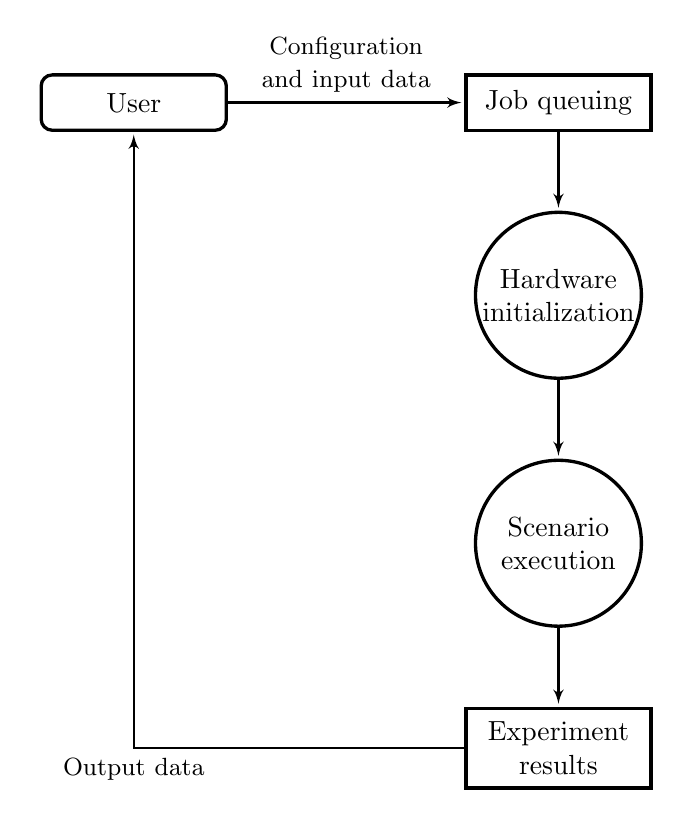
\begin{tikzpicture}[node distance=1cm, auto]
    \tikzset{
      circlenode/.style={circle,draw=black,very thick,inner sep=0em,minimum size=2cm,text width=2cm,text centered},
      rectroundnode/.style={rectangle,rounded corners,draw=black,very thick,inner sep=0.5em,minimum size=2em,text width=2cm,text centered},
      rectnode/.style={rectangle,draw=black,very thick,inner sep=0.5em,minimum size=2em,text width=2cm,text centered},
      label/.style={text width=7em,text centered},
      arrow/.style={->,>=latex',shorten >=1pt,thick}
    }
    \node[rectroundnode](user){User};
    \node[rectnode,right=3cm of user](queue){Job queuing};
    \node[circlenode,below=of queue](initialization){Hardware initialization};
    \node[circlenode,below=of initialization](job){Scenario execution};
    \node[rectnode,below=of job](results){Experiment results};

    \draw[arrow](user.east) -- node[label,above]{\small Configuration and input data} (queue.west);
    \draw[arrow](queue.south) -- (initialization.north);
    \draw[arrow](initialization.south) -- (job.north);
    \draw[arrow](job.south) -- (results.north);
    \draw[arrow](results.west) -| node[label,below]{\small Output data} (user.south);
  \end{tikzpicture}
  \medskip
  \caption{Basic experiment flow}
  \label{basic flow}
\end{figure}

Figure \ref{basic flow} shows the very basic experiment flow, based on the high-level functions.
The user submits the SDR Testbed configuration as well as experiment input data.
A job queuing mechanism queues the job for the user.
Once the job is picked up, the hardware is initialized, based on the configuration parameters.
The experiment scenario is executed using the input data provided.
As a final step, the result of the experiment is output and becomes available to the user.

\section{System Perspective}

\begin{figure}[H]
  \centering
  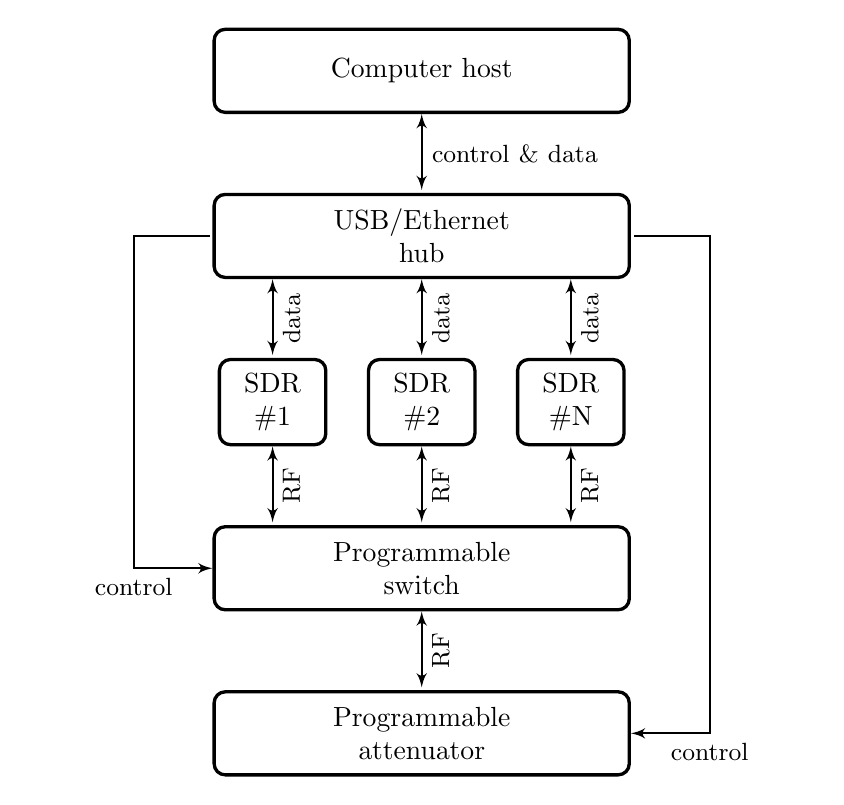
\begin{tikzpicture}[node distance=1cm, auto]
    \tikzset{
      rectroundnode/.style={rectangle,rounded corners,draw=black,very thick,inner sep=0.5em,minimum height=3em,text width=2.5cm,text centered},
      label/.style={text width=7em},
      arrow/.style={<->,>=latex',shorten >=1pt,thick}
    }
    \node[rectroundnode,minimum width=15em](host){Computer host};
    \node[rectroundnode,below=of host,minimum width=15em](hub){USB/Ethernet hub};
    \node[rectroundnode,below=of hub,text width=1cm](sdr2){SDR \#2};
    \node[rectroundnode,left=0.5cm of sdr2,text width=1cm](sdr1){SDR \#1};
    \node[rectroundnode,right=0.5cm of sdr2,text width=1cm](sdrn){SDR \#N};
    \node[rectroundnode,below=of sdr2,minimum width=15em](progswitch){Programmable switch};
    \node[rectroundnode,below=of progswitch,minimum width=15em](progatt){Programmable attenuator};

    \draw[arrow](host.south) -- node[label,right]{\small control \& data} (hub.north);
    \draw[arrow](hub.south) -- node[label,right]{\rotatebox{90}{\small data}} (sdr2.north);
    \draw[arrow](hub.south -| sdr1.north) -- node[label,right]{\rotatebox{90}{\small data}} (sdr1.north);
    \draw[arrow](hub.south -| sdrn.north) -- node[label,right]{\rotatebox{90}{\small data}} (sdrn.north);
    \draw[arrow](sdr2.south) -- node[label,right]{\rotatebox{90}{\small RF}} (progswitch.north);
    \draw[arrow](sdr1.south) -- node[label,right]{\rotatebox{90}{\small RF}} (progswitch.north -| sdr1.south);
    \draw[arrow](sdrn.south) -- node[label,right]{\rotatebox{90}{\small RF}} (progswitch.north -| sdrn.south);
    \draw[arrow](progswitch.south) -- node[label,right]{\rotatebox{90}{\small RF}} (progatt.north);
    \draw[arrow,<-](progswitch.west) -| ++(-1cm,0) node[label,below,text centered]{\small control} |- (hub.west);
    \draw[arrow,<-](progatt.east) -| ++(1cm,0) node[label,below,text centered]{\small control} |- (hub.east);

  \end{tikzpicture}
  \medskip
  \caption{Example hardware block diagram}
  \label{hardware block diagram}
\end{figure}

The SDR Testbed consists both of software and hardware components.
Figure \ref{hardware block diagram} shows an example high-level block diagram of the hardware components.
These components are:
\begin{itemize}
\item A computer host on which the SDR Testbed software will be running
\item A USB or/and Ethernet hub for the SDR devices and programmable RF components to connect with the host
\item A set of SDR devices
\item A set of programmable RF componets (e.g. RF switch, attenuators, etc.)
\item A set of fixed components (e.g. USB, Ethernet, RF cables and connectors, fixed attenuators, etc.)
\end{itemize}

As a whole, the SDR Testbed shall be an independent and totally self-contained system and not part of a larger system.
Thus, no strict requirements for external interfaces are set.
Nevertheless, additional ready-made components not defined in this specification may be used to complete it.

\section{Operating Environment}

The software operating environment will be based, to the maximum extent possible, on free and open source software.
All software components of SDR Testbed will be running on Linux OS.
It is suggested that a modern enterprise grade Linux distribution (e.g. CentOS) should be used for this purpose.
The services and application will be containerized to provide isolation and easier management.

The hardware operating environment can be based both on commercial and/or non-commercial hardware.
The testbed will be developed for x86-64 hardware platform, either server or COTS PC.
Nevertheless, provision has been made so that it will be possible to run on different architectures with minimal changes.
Most of the communication between hardware components will be over USB or IP network.

\section{Design and Implementation Constraints}

The following design and implementation constraints will be present on the SDR Testbed:
\begin{itemize}
\item Jobs will be queued and executed sequentially.
  The testbed can only handle a single experiment at a time.
  Nevertheless, scaling-out will be possible i.e. by adding more SDR Testbeds.
\item A limited number of SDR devices will be supported.
  Hardware restrictions place a limit on the number of devices which can be supported.
  A fixed number of USB and Ethernet ports will be available on the system for connecting SDR devices.
\item The duration of an experiment will be limited.
  Since the jobs will be executed sequentially, a limit on the duration of experiments will be placed.
\end{itemize}

\section{Documentation}

The documentation will consist of two parts:
\begin{itemize}
\item Users' documentation. This documentation will be the manual on how to use the testbed from users' point of view.
\item Developers' documentation. This documentation will be intended for developers on how to further extend or maintain the system.
\end{itemize}

\section{Assumption and Dependencies}

This system will be designed with the assumption that any experiment will not exceed the performance limits of the hardware.
This includes CPU power, RAM available, storage space, etc. as well as electrical characteristics (e.g. PSU or USB power available).
See chapter \ref{chapter_4} for more details.


\chapter{External Interfaces}
\section{User Interfaces}

The entry point of the user to the SDR Testbed shall be a Git repository.
The user shall commit:
\begin{itemize}
\item the scenario for an experiment.
  This scenario shall be written as a Robot Framework Suite.
\item raw data to be fed to the SDR devices.
  Git LFS shall be used to commit raw I/Q data.
\item configuration of the SDR Testbed hardware.
  The configuration includes selection of the SDR devices to be used and attenuation level.
\end{itemize}
The user shall push the commits to a remote Git repository managed by GitLab.
GitLab CI shall queue a job to be executed to the computer host where the SDR devices are attached.
After the execution and completion of the job, the host shall upload the results to the server managing the jobs.
The user shall be able to view and download the results of the experiment from the job server.

\section{Software Interfaces}

The SDR Testbed shall have the following software interfaces:
\begin{itemize}
\item an SDR development platform.
  GNU Radio shall be the platform which will be supported initially.
  Nevertheless, it shall be possible to support other platforms in the future (i.e. Pothos SDR).
\item VISA API and instrument drivers.
  VISA is a standard instrument control abstraction layer and shall be used to control the programmable RF switches and attenuators.
\item an SDR control and data interface.
  A new software interface shall be developed to abstract the control and data exchange towards the SDR application.
  This interface shall act as a wrapper function with a purpose to allow realtime control of the SDR during an experiment.
\item an experiment results file format interface.
  HDF5 file format shall be used to store the some experiment results.
  This interface is the library for supporting HDF5 storing.
\end{itemize}

\section{Hardware Interfaces}

\section{Communication Interfaces}


\chapter{Requirements} \label{chapter_4}
\section{Functional Requirements}

\section{Performance Requirements}

\section{Security Requirements}


\chapter*{Appendix I: Glossary and Acronyms}
\addcontentsline{toc}{chapter}{Appendix I: Glossary and Acronyms}

\printglossary
\printglossary[type=\acronymtype]

\end{document}
